%
% xtal formulas
% @author Tobias Weber <tweber@ill.fr>
% @date 13-jul-2018
% @license see 'LICENSE' file
%

In this chapter we review the theory for conversion between crystal coordinates and scattering angles at the triple-axis instrument. Section \ref{sec:xtalcoords} introduces crystal coordinates and the so-called UB matrix formalism, section \ref{sec:tasangles} calculates the corresponding TAS angles. Note this chapter has been published in the manual of the software from Ref. \cite{Takin2021} and is based on an earlier version of these derivations from my (physics) PhD thesis \cite{PhDWeber}.


% ------------------------------------------------------------------------------------------------------------------------------------
\section{Fractional crystal coordinates \label{sec:xtalcoords}}

We begin by presenting the so-called $UB$ matrix formalism to convert between relative lattice units of a crystal and laboratory coordinates used in instrument space. This method has been described in \cite{Lumsden2005}. The derivation of the transformation matrices, $A$ and $B$, describing fractional crystal coordinates, can be found in \cite{wiki_fractional}, which we follow here.

The unit cell of the crystal is spanned by its three basis vectors $\left| a \right>$, $\left| b \right>$, and $\left| c \right>$, which -- in general -- are not perpendicular to one another, but instead enclose angles of $\alpha$, $\beta$, and $\gamma$, respectively, as shown in Fig. \ref{fig:cell}. 
To calculate the crystallographic $A$ matrix which transforms non-orthogonal crystal to orthogonal lab units, we first need to reduce the number of parameters.
The respective relations between the basis vectors and their angles can be directly obtained via the cosine theorem:
\begin{equation} \left< a | b \right > \ =\  ab \cos \gamma, \label{ab} \end{equation}
\begin{equation} \left< a | c \right > \ =\  ac \cos \beta, \label{ac} \end{equation}
\begin{equation} \left< b | c \right > \ =\  bc \cos \alpha. \label{bc} \end{equation}

\begin{figure*}
	\centering
	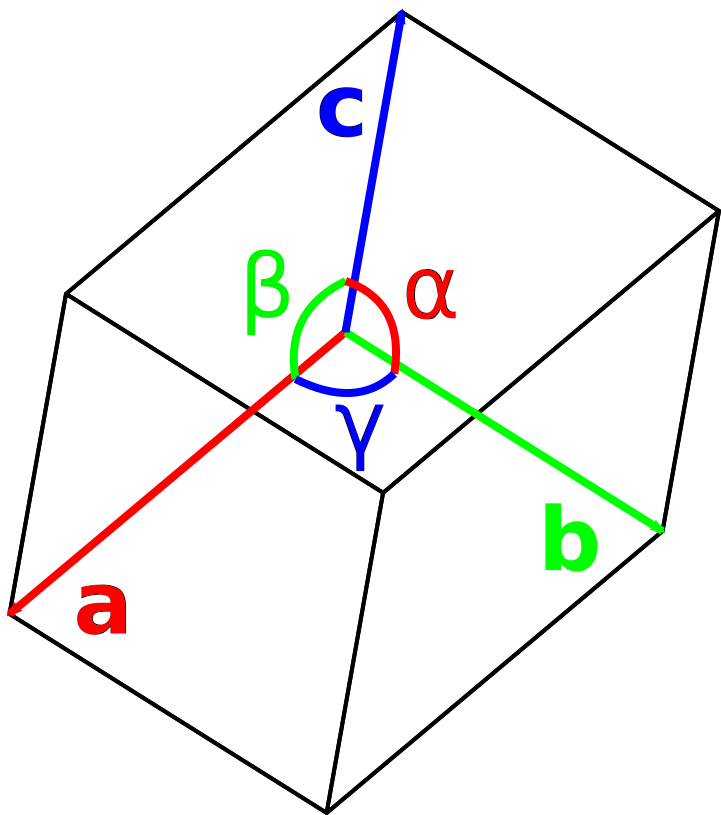
\includegraphics[width = 0.2 \textwidth]{figures/cell}
	\caption{The unit cell of a crystal is given by its coordinate vectors $a$, $b$, and $c$ 
		as well as their angles $\alpha$, $\beta$, and $\gamma$.}
	\label{fig:cell}
\end{figure*}


%\subsection*{Basis vectors}

The next goal is to explicitly write the components of the vectors $\left| a \right>$, $\left| b \right>$, and $\left| c \right>$ in terms of their (scalar) lengths $a = \sqrt{\left< a | a \right>}$, $b = \sqrt{\left< b | b \right>}$, $c = \sqrt{\left< c | c \right>}$, and the three angles.
To that end, we first choose -- without loss of generality -- $\left| a \right>$ along the $x$ axis, $\left| b \right>$ in the $xy$ plane, and $\left| c \right>$ in general:
\begin{equation} 
	\boxed{ \left| a \right> = \left( \begin{array}{c} a_1 = a \\ 0 \\ 0 \end{array} \right), }
	\hspace{0.5cm} \left| b \right> = \left( \begin{array}{c} b_1 \\ b_2 \\ 0 \end{array} \right),
	\hspace{0.5cm} \left| c \right> = \left( \begin{array}{c} c_1 \\ c_2 \\ c_3 \end{array} \right).
\end{equation}


Inserting $\left| a \right>$ and $\left| b \right>$ into Eq. \ref{ab} gives:

\begin{equation} \left< a | b \right > = a_1 b_1 = ab \cos \gamma, \end{equation}
\begin{equation} b_1 = b \cos \gamma. \end{equation}


Using the cross product between $\left| a \right>$ and $\left| b \right>$, we get:
\begin{equation} 
	\left\Vert \left| a \right> \times \left| b \right> \right\Vert =
	\left\Vert \left( \begin{array}{c} 0 \\ 0 \\ a_1 b_2 \end{array} \right) \right\Vert =
	ab \sin \gamma, \label{crossab}
\end{equation}
\begin{equation} b_2 = b \sin \gamma, \end{equation}
\begin{equation} 
\boxed{ \left| b \right> = \left( \begin{array}{c} b \cos \gamma \\ b \sin \gamma \\ 0 \end{array} \right). } 
\label{bvec} 
\end{equation}


Inserting $\left| a \right>$ and $\left| c \right>$ into Eq. \ref{ac} gives:

\begin{equation} \left< a | c \right > = a_1 c_1 = ac \cos \beta, \end{equation}
\begin{equation} c_1 = c \cos \beta. \end{equation}



Inserting $\left| b \right>$ and $\left| c \right>$ into Eq. \ref{bc} gives:

\begin{equation} \left< b | c \right > = b_1 c_1 + b_2 c_2 = bc \cos \alpha, \end{equation}
\begin{equation} b \cos \gamma \cdot c \cos \beta + b \sin \gamma \cdot c_2 = bc \cos \alpha, \end{equation}
\begin{equation} c_2 = \frac{c \cos \alpha - c \cos \gamma \cos \beta}{\sin \gamma}. \end{equation}



The last component, $c_3$, can be obtained from the vector length normalisation, $ \left< c | c \right> = c^2 $:
\begin{equation} \left< c | c \right > = c_1^2 + c_2^2 + c_3^2 = c^2, \end{equation}
\begin{equation} c_3^2 = c^2 - c_1^2 - c_2^2, \end{equation}
\begin{equation} 
	c_3^2 = c^2 \left[1 - \cos^2 \beta - \left(\frac{\cos \alpha - \cos \gamma \cos \beta}{\sin \gamma} \right)^2 \right], 
\end{equation}
\begin{equation} \boxed{ \left| c \right> = \left( \begin{array}{c}
	c \cdot \cos \beta \\
	c \cdot \frac{\cos \alpha - \cos \gamma \cos \beta}{\sin \gamma} \\
	c \cdot \sqrt{ \sin^2 \beta - \left(\frac{\cos \alpha - \cos \gamma \cos \beta}{\sin \gamma} \right)^2 }
\end{array} \right). } \end{equation}



The crystallographic $A$ matrix, which transforms real-space fractional to lab coordinates (\AA), is formed with the basis vectors in its columns:
\begin{equation}
	A = \left(
		\begin{array}{ccc}
			\left| a \right> & \left| b \right> & \left| c \right>
		\end{array}
	\right).
\end{equation}
The $B$ matrix, which transforms reciprocal-space relative lattice units (rlu) to lab coordinates (1/\AA), is:
\begin{equation} B = 2 \pi A^{-t}, \end{equation}
where $-t$ denotes the transposed inverse.
We can determine the metric tensor corresponding to the coordinate system defined by the $B$ transformation matrix, it reads \cite[p. 808]{Arens2015}:
\begin{equation}
	\left(g_{ij}\right) = \left<\underline{b}_i | \underline{b}_j \right> = B^T B,
\end{equation}
where the reciprocal basis vectors $\left| \underline{b}_i \right>$ form the columns of $B$.


\subsection*{Example: lengths and angles in the reciprocal lattice}
Having a metric makes it straightforward to calculate lengths and angles.
The length of a reciprocal lattice vector $\left| G \right>$ seen from the lab system is (in 1/\AA{} units) \cite[p. 808]{Arens2015}:
\begin{equation}
	\left\Vert \left< G | G \right> \right\Vert = \sqrt{\left< G | G \right>} = \sqrt{G_i G^j} = \sqrt{g_{ij} G^i G^j}.
\end{equation}
The angle $\theta$ between two Bragg peaks $\left| G \right>$ and $\left| H \right>$ is given by their dot product \cite[p. 808]{Arens2015}:
\begin{equation}
	\frac{\left< G | H \right>}{\left\Vert \left< G | G \right> \right\Vert \cdot \left\Vert \left< H | H \right> \right\Vert} = 
	\frac{g_{ij} G^i H^j }{\sqrt{g_{ij} G^i G^j} \sqrt{g_{ij} H^i H^j}} = \cos \theta.
\end{equation}
% ------------------------------------------------------------------------------------------------------------------------------------




% ------------------------------------------------------------------------------------------------------------------------------------
\section{Scattering triangle and TAS angles \label{sec:tasangles}}

The derivation of basic scattering geometries in triple-axis spectrometers can be found in \cite[Ch. 1.3]{Shirane2002}.

\begin{figure}
\begin{center}
	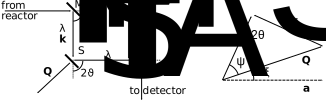
\includegraphics[width = 0.75 \textwidth]{figures/tas_triangle}
\end{center}
\caption{Triple-axis layout (left) and scattering triangle (right).}
\end{figure}


\subsection*{Monochromator angles $a_1$, $a_2$ and analyser angles $a_5$, $a_6$}

The monochromator (and analyser) angles follow directly from Bragg's equation:
\begin{equation} 2 d_{m,a}\sin a_{1,5} = n \lambda_{i,f}, \end{equation}
\begin{equation} 2 k_{i,f} \sin a_{1,5} = 2 \pi n / d_{m,a}, \end{equation}
\begin{equation} \boxed{ a_{1,5} = \arcsin \left( \frac{\pi n}{d_{m,a} \cdot k_{i,f}} \right). } \end{equation}

Fulfilling the Bragg condition, the angles $a_2$ and $a_6$ are simply: $a_{2,6} = 2 \cdot a_{1,5}.$



\subsection*{Scattering angle $a_4$}

\begin{equation} 
	\left| Q \right> = \left| k_i \right> - \left| k_f \right> \\ 
\end{equation}
\begin{equation} 
	\left< Q | Q \right> = \left( \left< k_i \right| - \left< k_f \right| \right) \cdot \left( \left| k_i \right> - \left| k_f \right> \right)
\end{equation}
\begin{equation} 
	\left< Q | Q \right> = \left< k_i | k_i \right> + \left< k_f | k_f \right> - 2 \left< k_i | k_f \right> 
\end{equation}
\begin{equation} 
	Q^2 = k_i^2 + k_f^2 - 2 k_i k_f \cos a_4 
\end{equation}
\begin{equation}
	\boxed{ a_4 = \sigma_s \cdot \arccos \left( \frac{k_i^2 + k_f^2 - Q^2}{2 k_i k_f} \right) } 
\end{equation}

The sign of $a_4$ is given by the sample scattering sense $\sigma_s = \pm 1$.




\subsection*{Rocking angle $a_3$}

\begin{equation} \boxed{ a_3 = 180^{\circ} - \left( \psi + \xi \right) } \end{equation}


\subsubsection*{Angle $\psi$}
Angle $\psi$ between $\left| k_i \right>$ and $\left| Q \right>$, in units of \AA{}$^{-1}$, as before:
\begin{equation}
	\left| k_f \right> = \left| k_i \right> - \left| Q \right> 
\end{equation}
\begin{equation} 
	\left< k_f | k_f \right> = \left( \left< k_i \right| - \left< Q \right| \right) \cdot \left( \left| k_i \right> - \left| Q \right> \right)
\end{equation}
\begin{equation}
	\left< k_f | k_f \right> = \left< k_i | k_i \right> + \left< Q | Q \right> - 2 \left< k_i | Q \right>
\end{equation}
\begin{equation}
	k_f^2 = k_i^2 + Q^2 - 2 k_i Q \cos \psi 
\end{equation}
\begin{equation}
	\boxed{ \psi = \sigma_s \cdot \arccos \left( \frac{k_i^2 + Q^2 - k_f^2}{2 k_i Q} \right) }
\end{equation}


\subsubsection*{Angle $\xi$}
Angle $\xi$ between $\left| Q \right>$ and orientation vector $\left| a \right>$ (i.e. $ax$, $ay$, $az$), in units of rlu:
\begin{equation} 
	\boxed{ \xi = 
\sigma_{\mathrm{side}} \cdot \arccos \left( \frac{ \left< Q | a \right> }{ \sqrt{\left< Q | Q \right>} \sqrt{\left< a | a \right>} } \right) = 
\sigma_{\mathrm{side}} \cdot \arccos \left( \frac{ Q^i g_{ij} a^j }{ \sqrt{Q^i g_{ij} Q^j} \sqrt{a^i g_{ij} a^j} } \right) } 
\end{equation}

The sign, $\sigma_{\mathrm{side}}$, of $\xi$ depends on which side of the orientation vector $\left| a \right>$ 
the scattering vector $\left| Q \right>$ is located. 
The sign can be found by calculating the (covariant) cross product of $\left| a \right>$ and $\left| Q \right>$ 
to give an out-of-plane vector $\left| x \right>$ which can be compared with the given scattering plane up vector. 
The covariant cross-product is calculated as \cite[p. 815]{Arens2015}:
\begin{equation}
	x^l = g^{li} \epsilon_{ijk} a^j Q^k, \hspace{0.5cm} \mathrm{with} \ 
	\epsilon_{ijk} = \left|
		\begin{array}{ccc} \left| 
			\underline{b}_i \right> & \left| \underline{b}_j \right> & \left| \underline{b}_k \right>
		\end{array} \right|.
\end{equation}


\paragraph*{Special case}
Special case for cubic crystals, $g_{ij} = \delta_{ij} \cdot \left( 2\pi / a \right)^2$:
\begin{equation}
	\xi = \sigma_{\mathrm{side}} \cdot \arccos \left( \frac{ Q_i a^i }{ \sqrt{Q_i Q^i} \sqrt{a_i a^i} } \right) 
\end{equation}
% ------------------------------------------------------------------------------------------------------------------------------------
